% GNUPLOT: LaTeX picture with Postscript
\begingroup
  \makeatletter
  \providecommand\color[2][]{%
    \GenericError{(gnuplot) \space\space\space\@spaces}{%
      Package color not loaded in conjunction with
      terminal option `colourtext'%
    }{See the gnuplot documentation for explanation.%
    }{Either use 'blacktext' in gnuplot or load the package
      color.sty in LaTeX.}%
    \renewcommand\color[2][]{}%
  }%
  \providecommand\includegraphics[2][]{%
    \GenericError{(gnuplot) \space\space\space\@spaces}{%
      Package graphicx or graphics not loaded%
    }{See the gnuplot documentation for explanation.%
    }{The gnuplot epslatex terminal needs graphicx.sty or graphics.sty.}%
    \renewcommand\includegraphics[2][]{}%
  }%
  \providecommand\rotatebox[2]{#2}%
  \@ifundefined{ifGPcolor}{%
    \newif\ifGPcolor
    \GPcolortrue
  }{}%
  \@ifundefined{ifGPblacktext}{%
    \newif\ifGPblacktext
    \GPblacktexttrue
  }{}%
  % define a \g@addto@macro without @ in the name:
  \let\gplgaddtomacro\g@addto@macro
  % define empty templates for all commands taking text:
  \gdef\gplbacktext{}%
  \gdef\gplfronttext{}%
  \makeatother
  \ifGPblacktext
    % no textcolor at all
    \def\colorrgb#1{}%
    \def\colorgray#1{}%
  \else
    % gray or color?
    \ifGPcolor
      \def\colorrgb#1{\color[rgb]{#1}}%
      \def\colorgray#1{\color[gray]{#1}}%
      \expandafter\def\csname LTw\endcsname{\color{white}}%
      \expandafter\def\csname LTb\endcsname{\color{black}}%
      \expandafter\def\csname LTa\endcsname{\color{black}}%
      \expandafter\def\csname LT0\endcsname{\color[rgb]{1,0,0}}%
      \expandafter\def\csname LT1\endcsname{\color[rgb]{0,1,0}}%
      \expandafter\def\csname LT2\endcsname{\color[rgb]{0,0,1}}%
      \expandafter\def\csname LT3\endcsname{\color[rgb]{1,0,1}}%
      \expandafter\def\csname LT4\endcsname{\color[rgb]{0,1,1}}%
      \expandafter\def\csname LT5\endcsname{\color[rgb]{1,1,0}}%
      \expandafter\def\csname LT6\endcsname{\color[rgb]{0,0,0}}%
      \expandafter\def\csname LT7\endcsname{\color[rgb]{1,0.3,0}}%
      \expandafter\def\csname LT8\endcsname{\color[rgb]{0.5,0.5,0.5}}%
    \else
      % gray
      \def\colorrgb#1{\color{black}}%
      \def\colorgray#1{\color[gray]{#1}}%
      \expandafter\def\csname LTw\endcsname{\color{white}}%
      \expandafter\def\csname LTb\endcsname{\color{black}}%
      \expandafter\def\csname LTa\endcsname{\color{black}}%
      \expandafter\def\csname LT0\endcsname{\color{black}}%
      \expandafter\def\csname LT1\endcsname{\color{black}}%
      \expandafter\def\csname LT2\endcsname{\color{black}}%
      \expandafter\def\csname LT3\endcsname{\color{black}}%
      \expandafter\def\csname LT4\endcsname{\color{black}}%
      \expandafter\def\csname LT5\endcsname{\color{black}}%
      \expandafter\def\csname LT6\endcsname{\color{black}}%
      \expandafter\def\csname LT7\endcsname{\color{black}}%
      \expandafter\def\csname LT8\endcsname{\color{black}}%
    \fi
  \fi
    \setlength{\unitlength}{0.0500bp}%
    \ifx\gptboxheight\undefined%
      \newlength{\gptboxheight}%
      \newlength{\gptboxwidth}%
      \newsavebox{\gptboxtext}%
    \fi%
    \setlength{\fboxrule}{0.5pt}%
    \setlength{\fboxsep}{1pt}%
\begin{picture}(10360.00,6900.00)%
    \gplgaddtomacro\gplbacktext{%
      \colorrgb{0.00,0.00,0.00}%%
      \put(922,3612){\makebox(0,0)[r]{\strut{}}}%
      \colorrgb{0.00,0.00,0.00}%%
      \put(922,4197){\makebox(0,0)[r]{\strut{}0.2}}%
      \colorrgb{0.00,0.00,0.00}%%
      \put(922,4781){\makebox(0,0)[r]{\strut{}0.4}}%
      \colorrgb{0.00,0.00,0.00}%%
      \put(922,5366){\makebox(0,0)[r]{\strut{}0.6}}%
      \colorrgb{0.00,0.00,0.00}%%
      \put(922,5950){\makebox(0,0)[r]{\strut{}0.8}}%
      \colorrgb{0.00,0.00,0.00}%%
      \put(922,6535){\makebox(0,0)[r]{\strut{}1}}%
      \colorrgb{0.00,0.00,0.00}%%
      \put(1473,3408){\makebox(0,0){\strut{}}}%
      \colorrgb{0.00,0.00,0.00}%%
      \put(2352,3408){\makebox(0,0){\strut{}}}%
      \colorrgb{0.00,0.00,0.00}%%
      \put(3231,3408){\makebox(0,0){\strut{}}}%
      \colorrgb{0.00,0.00,0.00}%%
      \put(4109,3408){\makebox(0,0){\strut{}}}%
      \colorrgb{0.00,0.00,0.00}%%
      \put(4988,3408){\makebox(0,0){\strut{}}}%
      \csname LTb\endcsname%%
      \put(3889,6243){\makebox(0,0)[l]{\strut{}Boltzmann}}%
    }%
    \gplgaddtomacro\gplfronttext{%
      \csname LTb\endcsname%%
      \put(400,5073){\rotatebox{-270}{\makebox(0,0){\strut{}Popolazione}}}%
    }%
    \gplgaddtomacro\gplbacktext{%
      \colorrgb{0.00,0.00,0.00}%%
      \put(5316,3612){\makebox(0,0)[r]{\strut{}}}%
      \colorrgb{0.00,0.00,0.00}%%
      \put(5316,4197){\makebox(0,0)[r]{\strut{}}}%
      \colorrgb{0.00,0.00,0.00}%%
      \put(5316,4781){\makebox(0,0)[r]{\strut{}}}%
      \colorrgb{0.00,0.00,0.00}%%
      \put(5316,5366){\makebox(0,0)[r]{\strut{}}}%
      \colorrgb{0.00,0.00,0.00}%%
      \put(5316,5950){\makebox(0,0)[r]{\strut{}}}%
      \colorrgb{0.00,0.00,0.00}%%
      \put(5316,6535){\makebox(0,0)[r]{\strut{}}}%
      \colorrgb{0.00,0.00,0.00}%%
      \put(5867,3408){\makebox(0,0){\strut{}}}%
      \colorrgb{0.00,0.00,0.00}%%
      \put(6746,3408){\makebox(0,0){\strut{}}}%
      \colorrgb{0.00,0.00,0.00}%%
      \put(7625,3408){\makebox(0,0){\strut{}}}%
      \colorrgb{0.00,0.00,0.00}%%
      \put(8504,3408){\makebox(0,0){\strut{}}}%
      \colorrgb{0.00,0.00,0.00}%%
      \put(9383,3408){\makebox(0,0){\strut{}}}%
      \csname LTb\endcsname%%
      \put(8504,6243){\makebox(0,0)[l]{\strut{}ZPE300}}%
    }%
    \gplgaddtomacro\gplfronttext{%
    }%
    \gplgaddtomacro\gplbacktext{%
      \colorrgb{0.00,0.00,0.00}%%
      \put(922,688){\makebox(0,0)[r]{\strut{}0}}%
      \colorrgb{0.00,0.00,0.00}%%
      \put(922,1273){\makebox(0,0)[r]{\strut{}0.2}}%
      \colorrgb{0.00,0.00,0.00}%%
      \put(922,1857){\makebox(0,0)[r]{\strut{}0.4}}%
      \colorrgb{0.00,0.00,0.00}%%
      \put(922,2442){\makebox(0,0)[r]{\strut{}0.6}}%
      \colorrgb{0.00,0.00,0.00}%%
      \put(922,3026){\makebox(0,0)[r]{\strut{}0.8}}%
      \colorrgb{0.00,0.00,0.00}%%
      \put(922,3611){\makebox(0,0)[r]{\strut{}0}}%
      \colorrgb{0.00,0.00,0.00}%%
      \put(1473,484){\makebox(0,0){\strut{}1000}}%
      \colorrgb{0.00,0.00,0.00}%%
      \put(2352,484){\makebox(0,0){\strut{}3000}}%
      \colorrgb{0.00,0.00,0.00}%%
      \put(3231,484){\makebox(0,0){\strut{}5000}}%
      \colorrgb{0.00,0.00,0.00}%%
      \put(4109,484){\makebox(0,0){\strut{}7000}}%
      \colorrgb{0.00,0.00,0.00}%%
      \put(4988,484){\makebox(0,0){\strut{}9000}}%
      \csname LTb\endcsname%%
      \put(4109,3319){\makebox(0,0)[l]{\strut{}Wigner}}%
    }%
    \gplgaddtomacro\gplfronttext{%
      \csname LTb\endcsname%%
      \put(400,2149){\rotatebox{-270}{\makebox(0,0){\strut{}Popolazione}}}%
      \csname LTb\endcsname%%
      \put(3230,178){\makebox(0,0){\strut{}Tempo, fs}}%
      \csname LTb\endcsname%%
      \put(4562,2637){\makebox(0,0)[r]{\strut{}Indissociate}}%
      \csname LTb\endcsname%%
      \put(4562,2393){\makebox(0,0)[r]{\strut{}Prima dissociazione}}%
      \csname LTb\endcsname%%
      \put(4562,2149){\makebox(0,0)[r]{\strut{}Seconda dissociazione}}%
      \csname LTb\endcsname%%
      \put(4562,1905){\makebox(0,0)[r]{\strut{}S_0 trans}}%
      \csname LTb\endcsname%%
      \put(4562,1661){\makebox(0,0)[r]{\strut{}S_0 cis}}%
    }%
    \gplgaddtomacro\gplbacktext{%
      \colorrgb{0.00,0.00,0.00}%%
      \put(5316,688){\makebox(0,0)[r]{\strut{}}}%
      \colorrgb{0.00,0.00,0.00}%%
      \put(5316,1273){\makebox(0,0)[r]{\strut{}}}%
      \colorrgb{0.00,0.00,0.00}%%
      \put(5316,1857){\makebox(0,0)[r]{\strut{}}}%
      \colorrgb{0.00,0.00,0.00}%%
      \put(5316,2442){\makebox(0,0)[r]{\strut{}}}%
      \colorrgb{0.00,0.00,0.00}%%
      \put(5316,3026){\makebox(0,0)[r]{\strut{}}}%
      \colorrgb{0.00,0.00,0.00}%%
      \put(5316,3611){\makebox(0,0)[r]{\strut{}}}%
      \colorrgb{0.00,0.00,0.00}%%
      \put(5867,484){\makebox(0,0){\strut{}1000}}%
      \colorrgb{0.00,0.00,0.00}%%
      \put(6746,484){\makebox(0,0){\strut{}3000}}%
      \colorrgb{0.00,0.00,0.00}%%
      \put(7625,484){\makebox(0,0){\strut{}5000}}%
      \colorrgb{0.00,0.00,0.00}%%
      \put(8504,484){\makebox(0,0){\strut{}7000}}%
      \colorrgb{0.00,0.00,0.00}%%
      \put(9383,484){\makebox(0,0){\strut{}9000}}%
      \csname LTb\endcsname%%
      \put(8064,3319){\makebox(0,0)[l]{\strut{}Wigner.rid}}%
    }%
    \gplgaddtomacro\gplfronttext{%
      \csname LTb\endcsname%%
      \put(7625,178){\makebox(0,0){\strut{}Tempo, fs}}%
    }%
    \gplbacktext
    \put(0,0){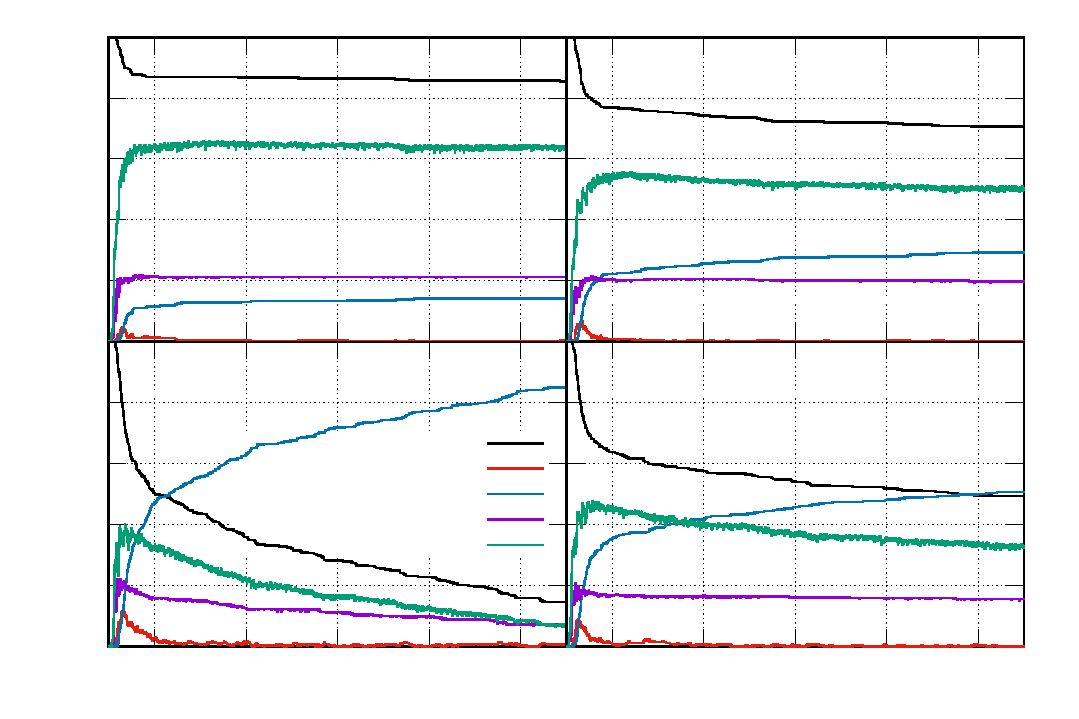
\includegraphics[width={518.00bp},height={345.00bp}]{presdisstot}}%
    \gplfronttext
  \end{picture}%
\endgroup
